% !TeX root = ../main-english.tex
% !TeX spellcheck = en-US
% !TeX encoding = utf8
% -*- coding:utf-8 mod:LaTeX -*-

%This smart spell only works if no changes have been made to the chapter
%using the options proposed in preambel/chapterheads.tex.
\setchapterpreamble[u]{%
	\dictum[John Claerbout, paraphrased by Buckheit \& Donoho]{An article about computational science in a scientific publication is not the scholarship itself, it is merely advertising of the scholarship. The actual scholarship is the complete software development environment and the complete set of instructions which generated the figures.}
}

\chapter{Introduction}
\label{chap:k1}

Look mom, some text!

\section{Brain state spaces}
This is an introduction into brain states and functional alignment
\pagebreak

\section{Magnetoencephalograpy (MEG)}
This is an introduction into \gls{meg} data

%The signals MEG measures are summed up postsynaptic potentials (IPSP or EPSP, slow-ish ~10ms and monophasic) that primarily originate from synchronized tangential neural activity produced by the parallel pyramidal cells that are perpendicular to the cortical sheet of the gray matter, mostly from the walls of the cortical sulci. The potential differences between soma and axons of neurons form magnetic dipoles, and, when aggregated across a neuronal population, measurable magnetic fields.
%The cortical magnetic fields produced by those signals are tiny, on the order of 10-10³ femtotesla (fT). This is a very weak magnetic field compared to the environmental noise.
%Magnetic flux is a measurement of the total magnetic field which passes through a given area, and is the physical measurement behind MEG.
%While active and passive shielding around the MEG measuring room are used for noise cancellation, flux transformers (input coils), placed as closely to the head as possible, amplify the magnetic field.
%Liquid helium in the dewar around the sensors cools the MEG down to -269°C and makes the flux transformer superconductive. In this state, there can’t be any net current in the flux transformer, and produce a more dense and stronger magnetic field that can be measured with Superconducting Quantum Interference Devices (SQUIDs) which are sensitive detectors of magnetic flux.
%Three main types of flux transformers exist: magnetometer, axial gradiometer, and planar gradiometer. Different flux transformers have a different sensitivity profile.

%Magnetometers are the most simple ones. They have a single coil and measure only one component of the magnetic field. This makes them very sensible to the distance of the source, but also susceptible to environmental noise.

%Gradiometers consist of two magnetometers placed in opposite directions. They exist in planar and axial orientation. Their general advantages are that environmental noise gets cancelled out and that they are as such more sensitive to the magnetic field of the cortical pyramidal sheet. An additional advantage of planar gradiometers is that their sensitivity is largest when placed directly over the dipol (a place where a magnetometer or axial can not pick up signals).
%Regardless of which flux transformer is used, MEG analysis consists of interpreting the resulting topographies given the employed flux transformer. Each flux transformer can be described by its lead field, i.e., how it couples to local source currents, which is very important information in source reconstruction.
%An MEG device can contain different types of flux transformers and the total number of flux transformers is the amount of channels of the MEG system.

%Typically, MEG devices contain around 150-300 sensors (SQUIDs) arranged in a helmet-shaped array that cover the whole human scalp at a frequency of 1000-5000Hz.
%This results in a typical temporal sampling rate of about ~1000Hz, and a typical spatial sampling rate of about ~300 sensors. The spatial topography of the activity is thus harder to pinpoint, but central in MEG analyses to make sense of the aggregated signal from multiple sources from within the brain at the scalp (a problem known as signal superposition - fields produced by several currents are sums of fields generated by each single current).




\pagebreak

\section{Research data management}
%This is an introduction on the importance of research data management for reproducible science

Research data encompasses everything that is produced in the life span of a research project.
From raw data acquisitions, preprocessed or otherwise standardized datasets, to software, analysis scripts, results, compiled reports or articles, figures, and other final or intermediate research outcomes.
To disambiguate the term ``research data'' from the smaller-scoped meaning of ``data'' in colloquial language (the outcome of a data acquisition in an experiment), it is also referred to as ``research objects``, and, in case it exists in purely electronic form, as ``digital research objects'' \citep{bechhofer2010research}. \\
Typically, research objects have a much longer life span than the project that creates them.
Science is an incremental process that produces and builds up on more than just published journal articles \citep{mons2018data}, and code, data, results, or tools of previous finished or unfinished projects fuel new undertakings.
\gls{rdm} describes the handling of these research objects through their entire life cycle: from curation, use, publication and sharing, archiving to re-use or destruction (\cref{fig:rdm-lifecycle}).
Ultimately, it ensures that research objects are preserved to act as an evidence base for findings, and as a discoverable resource for further reuse.
As I will lay out in this section and in upcoming chapters, \gls{rdm} is a foundational element within good scientific practice, and an important prerequisite for computational neuroscience.


\begin{figure}
	\centering
	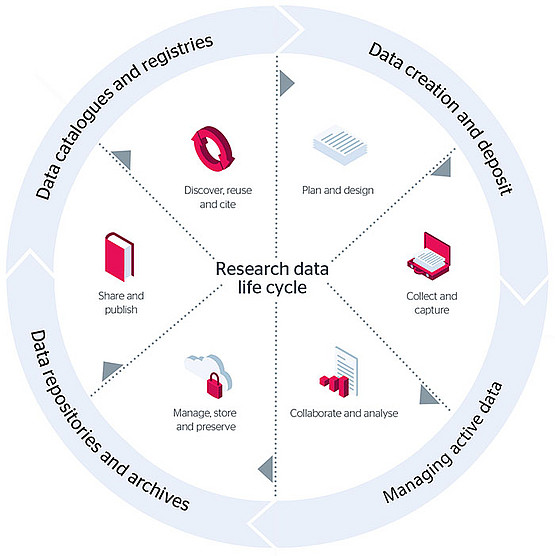
\includegraphics[width=.5\textwidth]{rdm-lifecycle-jisc.png}
	\caption[The life cycle of digital research objects]{The life cycle of digital research objects. License: JISC Research data management toolkit (\href{https://www.jisc.ac.uk/guides/rdm-toolkit}{www.jisc.ac.uk/guides/rdm-toolkit}), CC-BY-ND}
	\label{fig:rdm-lifecycle}
\end{figure}


\subsection{The FAIR guiding principles for scientific data management and stewardship}

Since their publication, the so-called \glsunset{FAIR}\gls{FAIR} principles \citep{wilkinson2016fair} have become guidelines for \gls{rdm} efforts for digital research objects.
They describe four measurable properties of research data that -- the better they are fulfilled -- serve the ultimate goal to improve the discoverability and reusability of data by machines and humans alike \citep{wilkinson2016fair}.
The \gls{FAIR}ness of data can be improved on each of the four related but separable major characteristics that are behind the \gls{FAIR} acronym (taken verbatim from \citet{wilkinson2016fair}):

\begin{itemize}
	\item \textbf{F}indable: To be Findable, (meta)data  are assigned a globally unique and persistent identifier (F1); data are described with rich metadata (F2); metadata clearly and explicitly include the identifier of the data it describes (F3);  (meta)data are registered or indexed in a searchable resource (F4)
	\item \textbf{A}ccessible: To be Accessible, (meta)data are retrievable by their identifier using a standardized communications protocol (A1); the protocol is open, free, and universally implementable (A1.1); the protocol allows for an authentication and authorization procedure, where necessary (A1.2);  metadata are accessible, even when the data are no longer available (A2)
	\item \textbf{I}nteroperable:  To be Interoperable, (meta)data use a formal, accessible, shared, and broadly applicable language for knowledge representation (I1); (meta)data use vocabularies that follow FAIR principles (I2); (meta)data include qualified references to other (meta)data (I3); and
	\item \textbf{R}eusable: To be Reusable, meta(data) are richly described with a plurality of accurate and relevant attributes (R1); (meta)data are released with a clear and accessible data usage license (R1.1); (meta)data are associated with detailed provenance (R1.2); (meta)data meet domain-relevant community standards (R1.3)
\end{itemize}

A pivotal factor for the importance of the FAIR principles is the increasing digitization of research practice, and with it, a rapid growth in research data \citep{dfg}.
Innovation relies on the ability to integrate new and existing data, and where the amount of data to discover, understand, and consolidate requires automation, research objects themselves need to become self-descriptive.
For this, the term ``machine-actionable'' is central to the \gls{FAIR} principles.
It is used to describe an ideal state in which a digital object provides detailed information (metadata) to an autonomously-acting, computational data explorer in two possible contexts: For one, as metadata about the object (``What is it?''), and second, as metadata about its content (``How do I process it?'') \citep{wilkinson2016fair}.
Importantly, the \gls{FAIR} principles do not suggest specific metadata standards, implementations, or technology choices.
But the end state of good \gls{rdm} for any digital research object is thus a high quality digital publication that facilitates and simplifies its discovery, evaluation, and reuse in downstream studies.\\
This reusability refers to the further use or utilization inside or outside its original research context, by the original author or different actors.
It is arguably the most important feature of a research object for various stakeholders: It can make research more efficient, foster collaborations, and speed up progress, and as it can reduce duplicate efforts it constitutes an economical benefit for funders as well as the public and industry \citep{nfdi2022data}.
Considering additional time spent, cost of redundant storage, licensing costs, research retraction, double funding, and missed potential for economic growth, the European Commission estimates that the cost of not having FAIR data lies between 10 and 26 billion euro per year \citep{eu2019FAIR}.
The largest position in their cost-benefit analysis is the time wasted by researchers when non-FAIR data takes more time to find, retrieve, clean, integrate, and peer review.
Together with the aspect of research retraction, the last point hints at an important side effect of good data management: Reproducibility.
Throughout this thesis, the connection between research data management and reproducibility will be exemplified.
The following sections will outline \gls{rdm} requirements and solutions in the field of neuroimaging that work towards this goal.


% Internationally accepted standard
%The largest funding institution for the sciences and humanities and research in Germany, the \gls{grf}, states that access to data and software according the the FAIR principles are of comparable importance to science as access to publications \citep{dfg}





\subsection{Research data management in neuroimaging}
\label{chap:k1-rdm-2}

%\[
%\left[
%\begin{tabular}{@{\quad}m{.3\textwidth}@{\qquad}m{.6\textwidth}@{\quad}}
%	\includegraphics[width=.7\linewidth]{qr_pub_niso.png} &
%	\raggedright%
%	\textbf{Related publications} \par
%	The following section contains a subset of the work presented in our original publication \citet{NISO2022119623}.
	%
%\end{tabular}
%\right]
%\]


Neuroimaging data poses a number of additional challenges for research data management.
For one, the field is characterized by complex datasets.
They typically encompass different modalities (such as imaging, electro-physiological, and behavioral measurements) and often entail several recording sessions.
The \gls{BIDS} \citep{gorgolewski2016brain} is a community standard for organizing and describing neuroimaging data, and is widely considered as a successful solution for data standardization in such datasets.
It defines common and modality specific schemes for file names and file organization, file formats, and metadata to accompany raw or derived data.
An example of an \gls{meg} dataset, structured to \gls{BIDS} or organized idiosyncratically, is shown in \cref{fig:BIDS}.
\gls{BIDS} has widespread and growing support for different neuroimaging modalities, and is made a common prerequisite by neuroscientific data portals such as OpenNeuro \citep{markiewicz2021openneuro} or processing tools such as BIDSApps \citep{gorgolewski2017bids}.\\
The storage demands of neuroimaging data are not trivial, either.
\gls{BIDS} regulates which file formats must be used for which data type, and focuses on open file formats for accessibility and compression to reduce disk space requirements.
But neuroimaging data are nevertheless sizable \citep{van2014human}.
And a growing awareness that robust findings require sufficiently long recordings \citep{li2021moving} as well as large and representative samples \citep{button2013power, turner2018small} leads to large-scale datasets such as the Human Connectome Project \citep{van2013wu}, the Adolescent Brain Cognitive Development Study (ABCD) \citep{casey2018adolescent}, or the UK Biobank (UKB) project \citep{matthews2015uk} that pose infrastructural challenges for storage, analysis, transfer and archival.
Moreover, in human neuroimaging, data underlies strict data protection regulations such as the \gls{HIPAA} in the United States or the \gls{GDPR} in Europe.
This requires compliance to variable terms of data usage agreements, and often involves idiosyncratic processes to retrieve data \citep{waitedata}.\\
Processing of neuroimaging data usually involves multi-stepped workflows from acquisition through analysis to archival, and those frequently require several different software tools at every step \citep{poline2011, NISO2022119623}.
The amount of possible combinations of methods, parameters, and tools in neuroimaging analyses is thus large \citep{bowring2019exploring}.
But variations in analytic choices affect numeric results and conclusions \citep{silberzahn2018}.
In the field of task-based fMRI, \citet{botvinik2020variability} found highly variable conclusions when they instructed 70 independent research teams to analyze the same dataset with tools and methods of their choice to test the same hypotheses.
A similar project, EEGManyPipelines (\href{https://eegmanypipelines.org/}{eegmanypipelines.org}), is currently ongoing in the field of \gls{eeg}.
One central aspect \gls{rdm} thus needs to provide in neuroimaging is precise information about how tools, data, and actors were involved in the generation of a file.
This \textit{digital provenance}  (illustrated in \cref{fig:prov1}) is not meant to decrease the analytical variability.
Instead, it captures thorough, machine-actionable processing descriptions that are necessary to investigate differences between analysis outcomes, reproduce, or reuse them.
Despite reporting guidelines for MRI \citep{nichols2017best}, MEG \citep{pernet2020issues}, and EEG \citep{styles2021towards} studies, traditional publications still regularly fail to report all relevant details about recording, processing, and analysis  \citep[see, e.g.,][]{vsovskic2022better}.

%BIDS
\begin{figure}
	{\scriptsize
		\begin{minipage}{.49\textwidth}
			\begin{forest}
				pic dir tree,
				for tree={% kleiner Zeilenabstand
					s sep=0.02cm}
				[memento/
				[memento\_001/
				%		[Move\_correc\_SSS\_alignedinitial\_nonfitiso/
				%		[1\_memento\_001\_ml83-1\_mc\_transforminitial.fif, file]
				%		[2\_memento\_001\_ml83-1\_mc\_transforminitial.fif, file]
				%		[3\_memento\_001\_ml83-2\_mc\_transforminitial.fif, file]
				%		[data\_fix1.mat, file]
				%		[data\_fix\_ft1.mat, file]
				%		[data\_fix\_new1.mat, file]
				%		[data\_fix\_reduced1.mat, file]
				%		[delay\_photodiode\_subject\_long\_default\_realign\_only\_ICA1.mat, file]
				%		[memento\_results\_ICA\_newall\_alignedinitial228.mat, file]
				%		[memento\_results\_ICA\_newall\_alignedinitial461.mat, file]
				%		[memento\_results\_ICA\_newall\_alignedinitial511.mat, file]
				%		[num\_trials\_old\_ICA.mat, file]
				%		[resultfile\_probs-1.mat, file]
				%		[trial\_out\_ind.mat, file]
				%		]
				[Move\_correc\_SSS\_realigneddefault\_nonfittoiso/
				[1\_memento\_001\_ml83\_mc\_realigneddefault.fif, file]
				[2\_memento\_001\_ml83-1\_mc\_realigned\_default.fif, file]
				[3\_memento\_001\_ml83-1\_mc\_realigned\_default.fif, file]
				[memento\_results\_ICA228.mat, file]
				[memento\_results\_ICA455.mat, file]
				[memento\_results\_ICA461.mat, file]
				[memento\_results\_ICA511.mat, file]
				[memento\_results\_ICA\_newall228.mat, file]
				[memento\_results\_ICA\_newall455.mat, file]
				[memento\_results\_ICA\_newall461.mat, file]
				[memento\_results\_ICA\_newall511.mat, file]
				[mri\_aligned.mat, file]
				[num\_trials\_old\_ICA.mat, file]
				[outfile\_new\_all.mat, file]
				[resultfile\_new\_all.mat, file]
				[template\_grid.mat, file]
				[trial\_out\_ind.mat, file]
				]
				[Raw/
				[1\_memento\_001\_ml83.fif, file]
				[2\_memento\_001\_ml83-1.fif, file]
				[memento\_001\_ml83-2.fif, file]
				]
				]
				]
			\end{forest}
		\end{minipage}
		\quad
		\begin{minipage}{.49\textwidth}
			\begin{forest}
				pic dir tree,
				for tree={% kleiner Zeilenabstand
					s sep=0.02cm}
				[memento/
				[dataset\_description.json, file]
				[participants.json, file]
				[participants.tsv, file]
				[README, file]
				[sub-001/
				[meg/
				[sub-001\_acq-calibration\_meg.dat, file]
				[sub-001\_acq-crosstalk\_meg.fif, file]
				[sub-001\_coordsystem.json, file]
				[sub-001\_task-memento\_channels.tsv, file]
				[sub-001\_task-memento\_events.tsv, file]
				[sub-001\_task-memento\_log.tsv, file]
				[sub-001\_task-memento\_meg.json, file]
				[sub-001\_task-memento\_split-01\_meg.fif, file]
				[sub-001\_task-memento\_split-02\_meg.fif, file]
				[sub-001\_task-memento\_split-03\_meg.fif, file]
				]
				[sub-001\_scans.tsv, file]
				]
				]
			\end{forest}
		\end{minipage}
	}
	\caption[An example of BIDS]{A real-world example of a single subject's MEG acquisition. The left side shows the file tree of the data from a project directory with an idiosyncratic organization. It includes a mix of raw data, preprocessed data, and intermediate results, and the naming scheme is inconsistent. The right side shows the same subject's data, but structured according to \gls{BIDS}. The naming scheme is consistent, and apart from raw MEG data the directory includes metadata files from the experiment and acquisition machine that are required to understand the data without the original authors.}
	\label{fig:BIDS}
\end{figure}


% provenance
\begin{figure}
	\centering
	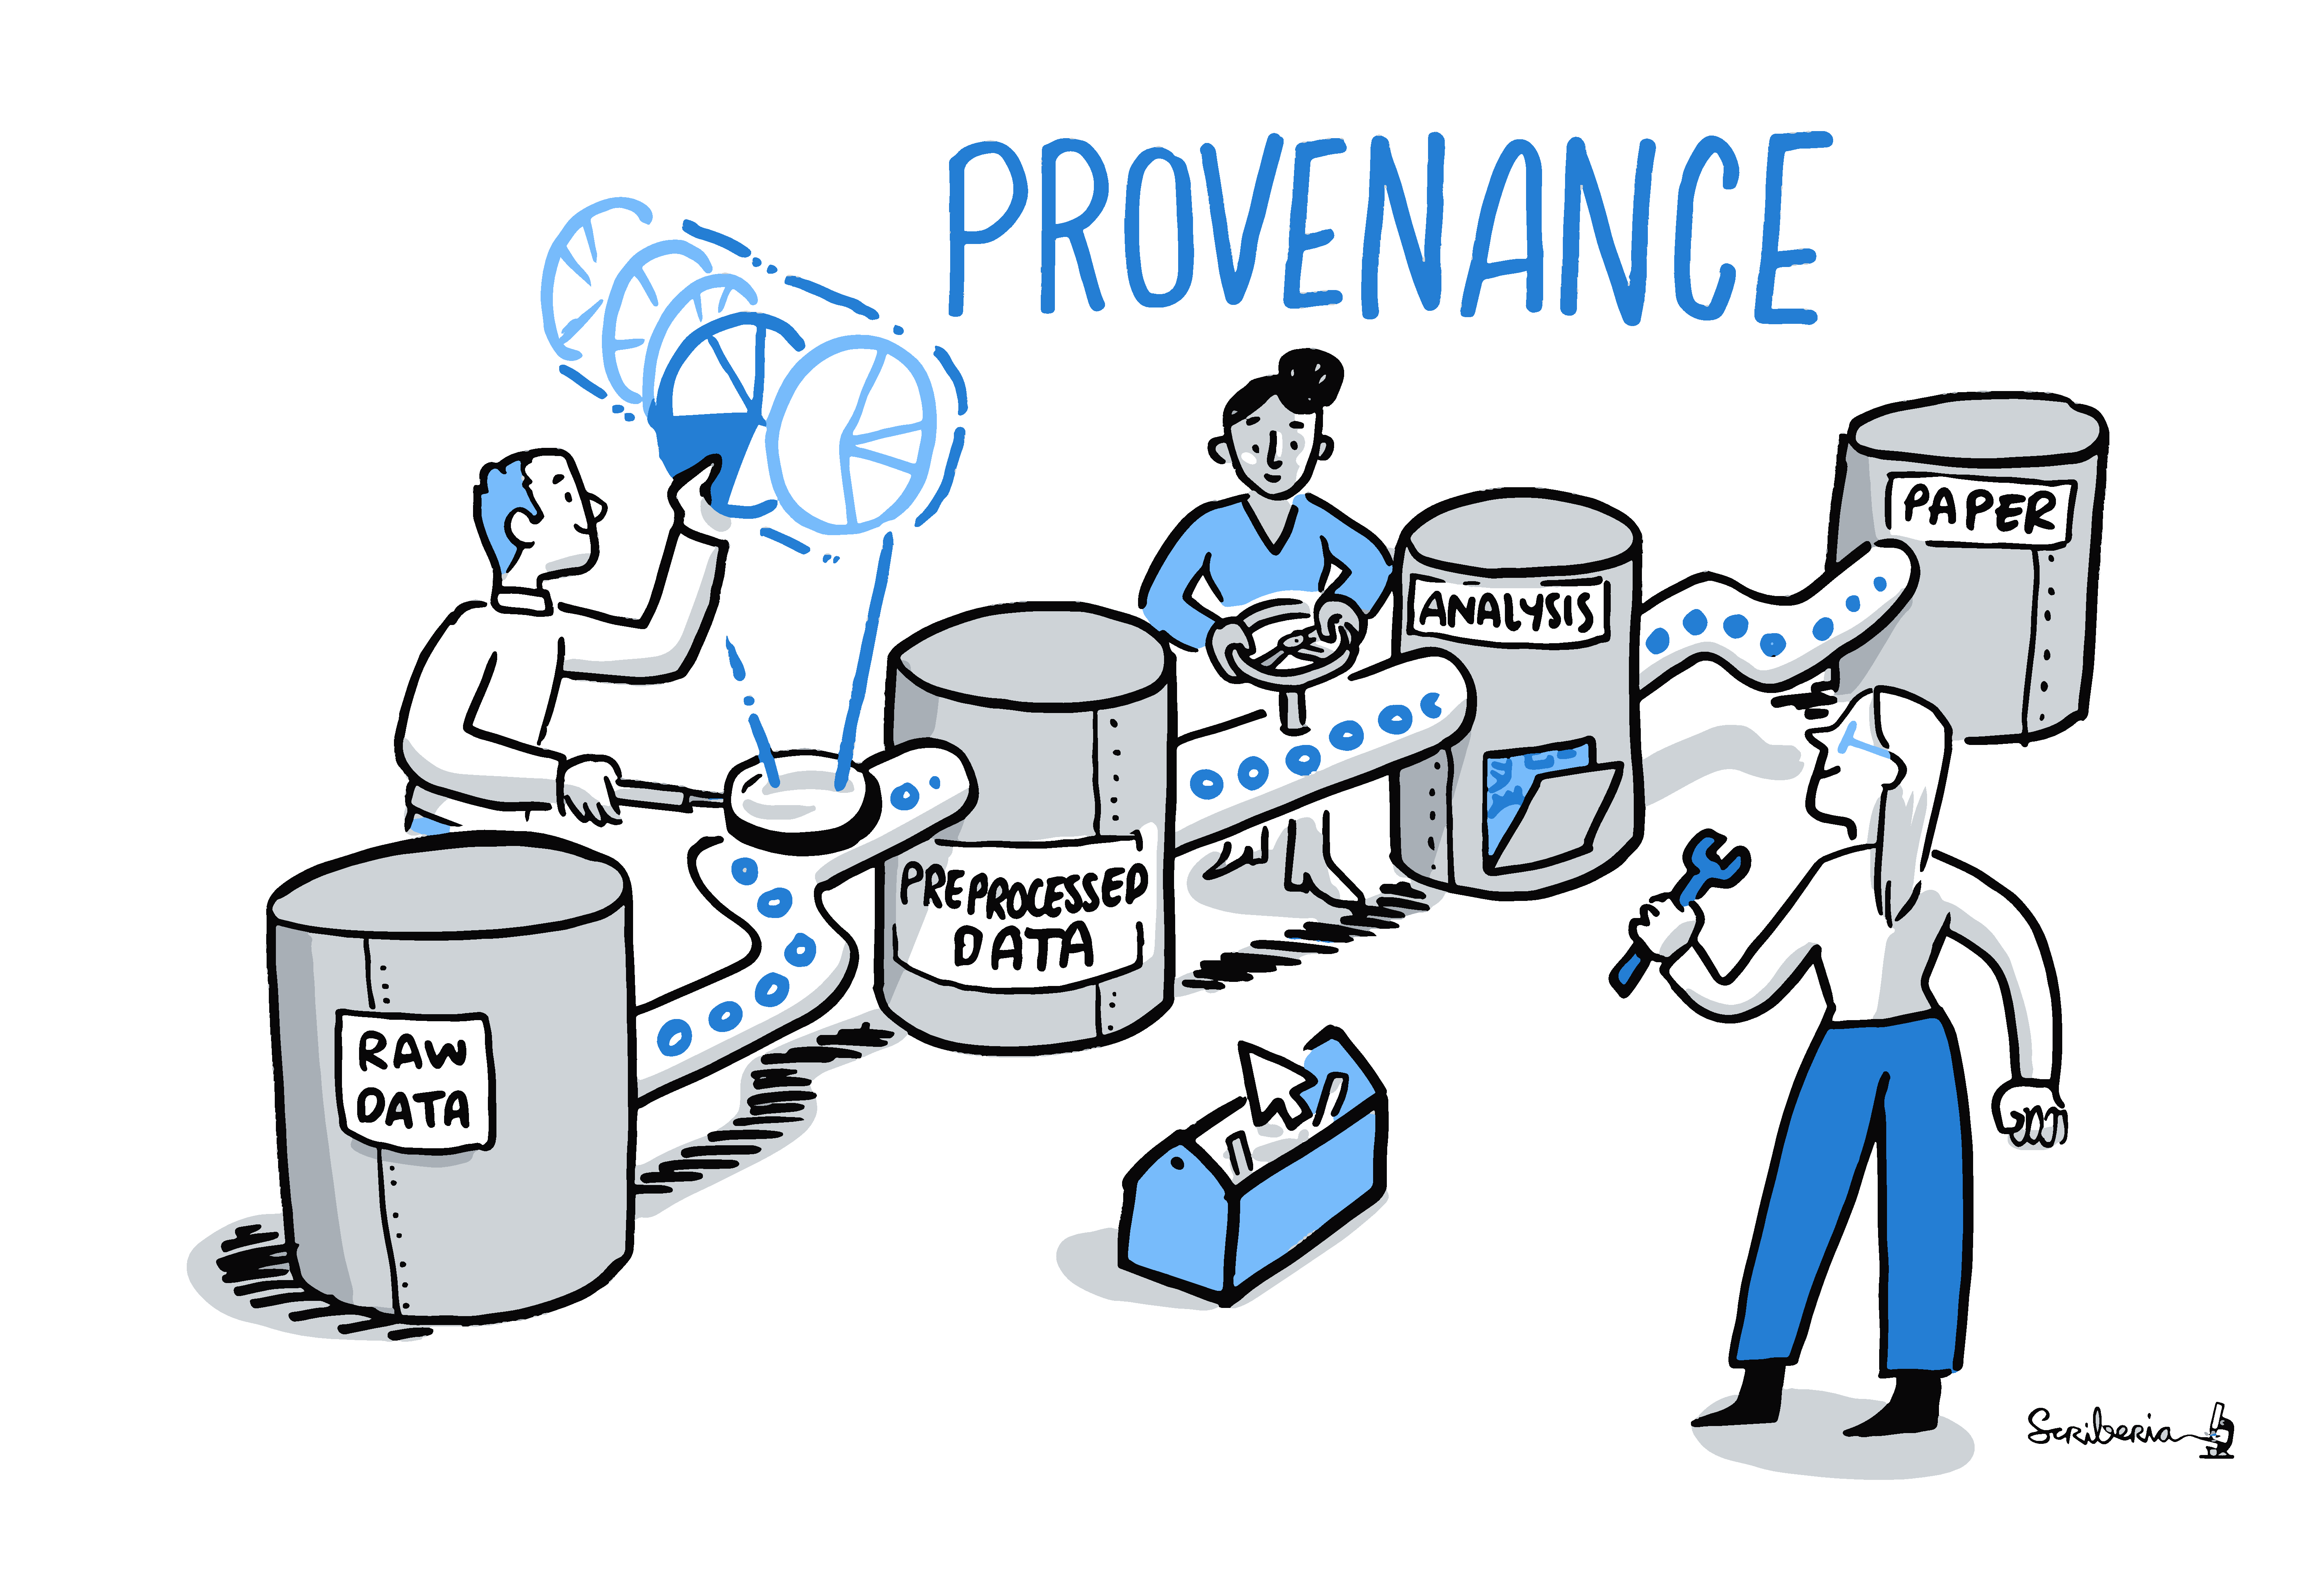
\includegraphics[width=.5\textwidth]{provenance.pdf}
	\caption[Provenance throughout the research process]{In multi-stepped analyses, a variety of choices affect the final outcome. Digital provenance, information about how tools, data, and actors were involved in the generation of file, is required to retrace, understand, and trust the decisions that led to a research outcome. Such provenance can be an outcome of good research data management. License: Scriberia and the Turing Way Project, CC-BY}
	\label{fig:prov1}
\end{figure}


\todo{add more RDM peculiarities of neuroimaging here. Maybe deep dive into computational modelling}

Careful \gls{rdm} is necessary to translate complex data efficiently into scientific insights.
Given these specific complexities in neuroimaging, solutions to these challenges often arise from the community of researchers.
The following section will highlight one of several software tools that aids with the complex task of research data management: DataLad.
A subsequent chapter, \cref{chap:k2}, will later focus on how research data management is a prerequisite of reproducible research, specifically with regards to software environments and large sample sizes.
In addition, \cref{chap:k2} will highlight pragmatic approaches to \gls{rdm} that can be embedded in standard research practice and contribute to the FAIRification of data, even in absence of established metadata formats.



% link to chapter 3: Research data management is a prerequisite of reproducible research

\section{DataLad as a software solution for research data management challenges}

%\[
%\left[
%\begin{tabular}{@{\quad}m{.3\textwidth}@{\qquad}m{.6\textwidth}@{\quad}}
%	\includegraphics[width=.7\linewidth]{qr_pub_datalad.png} &
%	\raggedright%
%	\textbf{Related publications} \par
	The following section provides an overview of the features of the software tool DataLad and their use for research data management.
	The reader is invited to refer to our original publication \citep{Halchenko2021} for a more detailed description.%
%\end{tabular}
%\right]
%\]

%This introduces DataLad as a software solution for research data management

DataLad (\href{http://datalad.org}{datalad.org}) is a Python-based, MIT-licensed software tool for the joint management of code, data, and their relationship.
It builds up on git-annex, a versatile system for data logistics \citep{hessannex}, and Git, the industry standard for distributed version control.
To address the technical challenges of data management, data sharing, and digital provenance collection, it adapts principles of open-source software development and distribution to scientific workflows. \\
%Initially, DataLad development started with the idea to make data retrieval as easy as installing software with package managers on Unix-based operating systems\footnote{On a Debian system, a user can install thousands of software package with a single command such as \texttt{apt get install <package-name>}.}.
%Now, DataLad aims to make data management as easy as managing code \citep{Halchenko2021}.
DataLad's aim is ``to make data management as easy as managing code'' \citep{Halchenko2021}.
The latter benefits from a well-established ecosystem of tools, platforms, and processes.
The distributed version control tool Git provides the ability to track changes in small-sized, text-based files, and is a de-facto standard in collaborative software development. In 2022, 93.78\% of respondents in Stackoverflow's annual developer survey (\url{https://survey.stackoverflow.co}) reported to use it.
Hosting platforms for Git repositories such as GitHub (\url{https://github.com}), GitLab ({\url{https://gitlab.com}), or Gin (\url{https://gin.g-node.org}) have been developed to serve as facilitators for collaboration, discovery, and reuse.
In the scientific community it is widely recommended to employ version control for code to foster reproducibility \citep[e.g.,][]{sandve2013ten}, and it is established practice to develop and share research software and code using Git and Git hosting platforms \citep[e.g.,][]{nord2019towards, strupler2017reproducibility, bryan2018excuse, corti2019managing}.
But other components of scientific projects, such as data or computing environments, are not as transparently managed or accessible as code and software.
Digital research objects are usually stored in multiple different locations \citep{parsons2013research}, and their consumption is complicated by disconnected and non-interoperable hosting solutions:
Different storage services use different protocols, means of authentication, or other idiosyncrasies that require custom workflows.
Unlike code in software development, data tend not to be as precisely identifiable because data versioning is rarely or only coarsely practiced.
Yet over the course of a research project, often as part of the standard, multi-stepped processing workflow, data evolve and change just like code does:
Continued acquisitions enlarge the raw dataset; Transformations to -- likewise evolving -- community standards change file formats, dataset organization, or enrich available metadata; And continuous quality control processes or accidental findings can bring errors to light and improve datasets with fixes.
In the case that data or other research objects were subject to change over the course of a project, there is a need to identify which exact version has been used -- otherwise, the reproducibility of a result is threatened \citep{hardwicke2018data}.
Likewise, scientific computation is not reproducible enough, because data provenance is often incomplete and rarely automatically captured.
Last but not least, in the absence of standardized data packages, there is no uniform way to declare actionable
data dependencies and derivative relationships between inputs and outputs of a computation.
Consequentially, data needs to be kept alongside to results to ensure reproducibility, even if it is hosted elsewhere already.
Especially in the age of big data neuroscience \citep{bzdok2017inference}, downloads or storage of datasets can become infeasible \citep{horien2021hitchhiker, grisham2016proposed}.
And although projects might only draw insights from only a subset of a dataset, such as only specific modalities, tasks, or participants, a project has heavier disk space demands if the original dataset is only available as a bulk download.\\
DataLad aims to solve these issues by providing streamlined, transparent management of code, data, computing environments, and their relationship.
Its main features are
\begin{itemize}
	\item Version control for data of any size or type
	\item Streamlined procedures to consume, publish, and update  all elements of scientific projects, with interoperability adapters to established scientific and commercial tools and services
	\item Data linkage as precisely versioned, lightweight dependencies
	\item Actionable process provenance capture for arbitrary command execution that affords automatic re-execution.
\end{itemize}

\subsection{Technical features}

Fundamental to DataLad's functionality is the concept of the ``DataLad dataset'', DataLad's central data structure.
On a technical level, it is a joint Git and git-annex repository with additional metadata and features for scientific use cases added on top by DataLad.\\
Git excels at managing and collaborating on text files, and provides a powerful back bone to DataLad's features.
Git repositories and their history can be easily distributed as linked \textit{clones} to suitable infrastructure.
Locally, changes to files can be saved (\textit{committed}) and transferred (\textit{pushed}) to all clones of a repository, and remote revisions can be retrieved and integrated (\textit{pulled}).\\
However, Git is not designed to handle large or binary files.
Git-annex overcomes this limitation and adds support to track and transfer files of arbitrary size or type without placing their content into Git.
Instead, it places file content into a managed repository \textit{annex} and only commits a lightweight reference that encodes the file's name and content identity via content hash into Git.
This reference allows a decoupling of file content (handled by git-annex) and file name (tracked with Git), but retains the ability to transparently notice and track changes: If file content changes, the identity reference known to Git changes, too, and the version control system becomes aware of the modification.
The same mechanism guarantees file integrity at all times, and can for example detect corruption during transfer.
While Git keeps a reference of the content \textit{identity}, git-annex tracks content \textit{availability}, and manages data transport with an extensible set of protocols and set of hosting solutions to and from a local repository annex at a granularity of individual files. \\
DataLad, finally, extends Git and git-annex with easy to use modularization, re-executable annotation of changes, and targeted interfaces and interoperability adapters.
Modularization suits research workflows because they can produce projects with many files or heterogeneous nature, comprising different data sources or evolving data across different processing stages.
A modular structure into homogeneous or smaller components enables efficient reuse.
Extending Git’s submodule mechanism, DataLad allows to nest individual datasets via versioned linkage as lightweight dependencies, and provides seamless recursive operations across dataset boundaries.
With this, DataLad provides a ``monorepo''-like user experience in datasets with arbitrarily deep nesting, and makes it trivial to operate on individual files deep in the hierarchy or entire trees of datasets.
In DataLad datasets, DataLad supports executing any command and automatically capturing the command, the generated outputs or modification, and optionally all required input elements.
This information is saved as re-executable provenance in a structured annotation to a Git commit message.
In addition to providing reliable information about past command-line invocations, these machine-readable records make it possible to easily re-execute commands, for example to verify if a result is computationally reproducible or to apply an analog change to a different dataset state.
% Process provenance—how code and commands created results from input data in a particular computational environment—of any processing routine can be captured and stored in machine-readable, automatically re-executable records (Figure 2). These records are created by a datalad run command for the execution of a shell command, or a container invocation by datalad containers-run. Users need to supply the command, a software environment, input data, and optionally which results should be saved as parameters. DataLad’s execution wrappers retrieve inputs, initiate command execution, and save results together with a provenance record.
% Because such containers can be stored in image files, they can be tracked and precisely versioned like any other component of a DataLad dataset.

Being able to efficiently retrieve and update research objects across a variety of available storage options is an important part of \gls{rdm} \citep{borghi2018data}.
Git can already interact with other local or remote repositories via standard or custom network transport protocols, and git-annex readily provides access to a wide range of external data storage resources via a large set of protocols.
On top of this, DataLad implements support for additional services that require custom protocols, such as the \gls{osf} \citep{hanke2021dlosf}, and adds, for example, more fine-grained access (e.g. direct access to individual components contained in an archive hosted on cloud storage) or specialized services, such as XNAT \citep[\url{www.xnat.org},][]{halchenko2021xnat}.
With this approach, DataLad can help to overcome technological limitations of storage solutions, like file size or inode limits, or integrate seamlessly with technology that is already in use.



\subsection{User experience}

On the conceptual level, a DataLad dataset is an overlay structure to version control files of any size, track and publish files in a distributed fashion, and record, publish, and execute actionable provenance of files and file
transformations.
On a file system, it appears like a regular directory.
DataLad's commands aim to simplify standard workflows from Git, git-annex, or hosting services to make them more accessible to technical novices.
For example, committing a file into Git requires a \texttt{git add <file>} followed by a \texttt{git commit}, and annexing a file requires a \texttt{git annex add <file>} followed by a \texttt{git commit}, but a \texttt{datalad save <file>} performs either action, with automatic decision making whether the file is annexed or committed to Git.
Likewise, publishing a repository to hosting sites usually requires interactions in the hosting site's web interface, but DataLad provides a set of \texttt{create-sibling-<service>} commands that spare users the need to visit the hosting service.
Nevertheless, compatibility with all Git and git-annex functionality is retained, and users are free to chose their workflows.
DataLad's streamlined access to data enables users to utilize web sources, including all major cloud storage providers, paths on local or remote computational infrastructure, or neuroscientific data registries such as OpenNeuro \citep{markiewicz2021openneuro} for file storage.
At the same time, the separation of file content and file name separates actual data retrieval from a lean meta-data based representation.
Thus, datasets of arbitrary scale can be cloned, exposing file names and revision history of all contained files, and provide actionable access to its content at a fraction of their total size.
And in order to expose datasets for access, DataLad can use repository hosting infrastructure as access points to install data, without actually publishing data contents to these services.
Like Git and git-annex, DataLad is primarily developed as a command line tool, but a \gls{gui} exists as well (see \cref{fig:gooey}).

% provenance
\begin{figure}
	\centering
	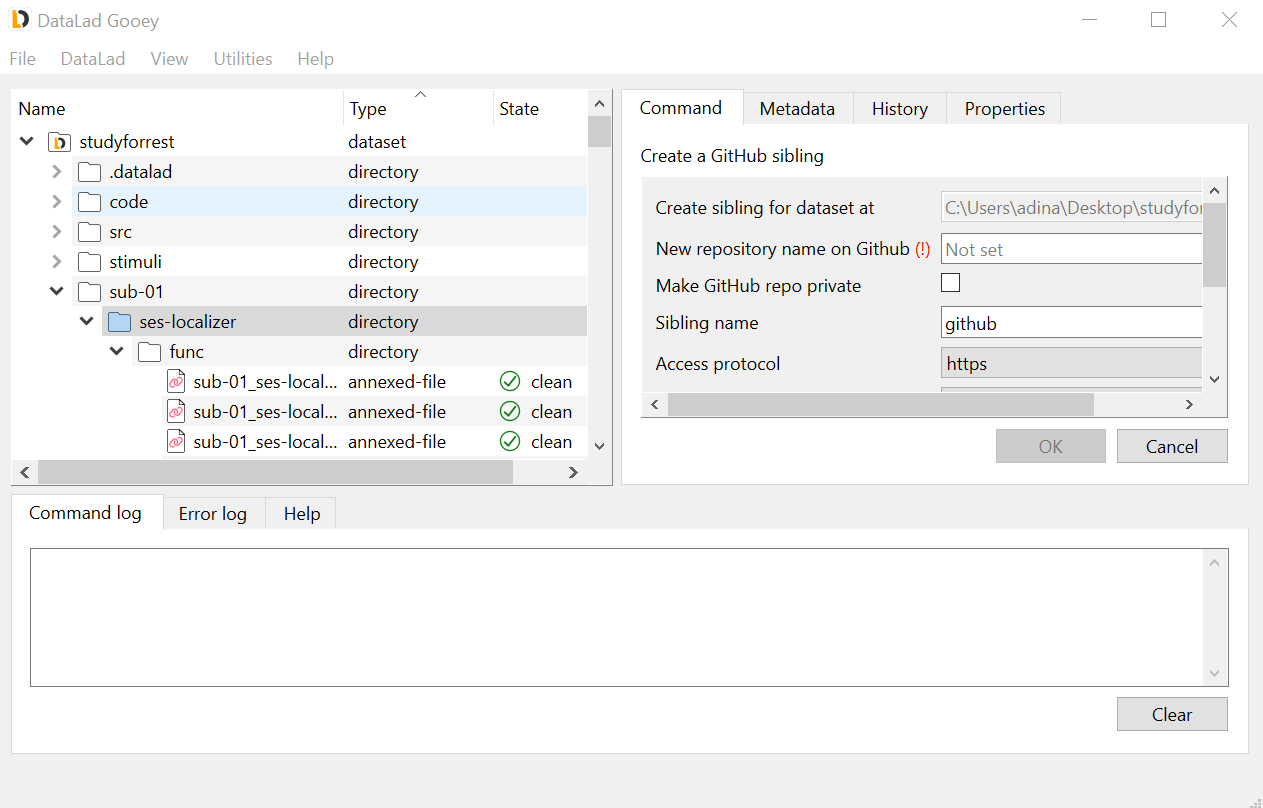
\includegraphics[width=.9\textwidth]{datalad_gooey.png}
	\caption[DataLad: Graphical User Interface]{The \gls{gui} of DataLad on a Windows system, provided by an extension package \texttt{datalad-gooey}. A file tree (left) provides an overview of the file system, and annotates elements into DataLad datasets, contents tracked with Git or git-annex, untracked, modified, or clean states. A command window (right) as well as right-click drop down menus (not shown) lets users parametrize and execute DataLad commands. A log window (bottom) can display result outcomes, error, or help text.}
	\label{fig:gooey}
\end{figure}


\subsection{Development principles}

DataLad's development is guided by four principles \citep{Halchenko2021}:
\begin{itemize}
	\item The only two recognized entities are Datasets and the files they comprise
	\item A dataset is a Git repository with an optional annex
	\item The should be as few custom procedures and data structures as possible
	\item Complete decentralization, with no required central server or service, but maximum interoperability with existing 3rd-party resources and infrastructure
\end{itemize}

These principles ensure DataLad's open and domain agnostic nature, maximize the long-term utility of DataLad datasets, minimize users’ technical debt and reduce the risk of adoption.
When using DataLad datasets as a standard package for digital objects, access to any resources managed with DataLad has no critical dependency on service deployments governed by central entities, and even on DataLad itself.
DataLad is further developed as an extensible ecosystem of software packages.
A core package provides basic functionality, and DataLad extensions, stand-alone Python packages with additional DataLad functionality, can extend it with domain-focused or technology-specific features.




% 5.2.1. WHAT
%Primary or preprocessed data form the basis of scientific analyses and insights. Flexible storage options and means for retrieval and updating of data are crucial for its further use. DataLad (Hanke et al., 2021) is a general purpose tool for managing and version controlling digital files in a decentralized manner, developed by a US-German collaboration in computational neuroscience. It can assist with storing and retrieving your own or other’s data in a transparent and streamlined fashion, and updating shared copies of data on demand. Based on the principle of maximizing interoperability with existing solutions, it aims to standardize data access and updates across hosting solutions.
%5.2.2. WHY
%
%5.2.3. WHERE
%DataLad can retrieve public data from major providers such as OpenNeuro (OpenNeuro.org), the Canadian Open Neuroscience Platform (conp.ca), the International Neuroimaging Data-sharing Initiative (INDI), the Healthy Brain Network Serial Scanning Initiative (HBN-SSI), Data sharing for Collaborative Research in Computational Neuroscience (CRCNS.org), the Human Connectome Project's open access dataset (Van Essen et al., 2013), and many more. Beyond public data, it can - given appropriate permissions or authentication - retrieve data from web-based storage providers, and local and remote paths. Information about DataLad can be found at datalad.org and in the DataLad Handbook (Wagner et al., 2021).
%5.2.4. HOW (and when)
%The demand for storage and retrieval exists throughout and beyond a scientific project, but changes frequently, depending on the type of data and the project stage. DataLad represents any data in a scalable, domain-agnostic overlay structure that can be exposed to standard services, but also moved across or distributed across sites or services, depending on current needs.



\subsection{Software adoption and relevance}

As DataLad does not employ tracking code, the exact number of its users is not known.
However, download statistics from the major Python package managers \texttt{pip} and \texttt{conda}, and popularity statistics from users of the Debian operating system can provide rough references.
According to pypistats.org, the main DataLad Python package was downloaded from the Python Package Index 300 times per day on average in May 2023.
The Python distribution Anaconda (anaconda.org) counts a total of 333932 downloads of the software throughout versions 0.9.3 (April 2018) and 0.18.3 (May 2023), averaging 180 downloads per day.
The \texttt{popularity-contest} software is a Debian package that, if installed on a users system, reports anonymous statistics about most-used Debian packages.
This data is aggregated into a popularity contest.
According to it, in May 2023 between 0.04 and 0.05 percent of systems reporting statistics have an installation of the DataLad Debian package, or the equivalent python3-datalad Debian package.
All of these sources contain biases that limit conclusion to the number of users, though.
Installations via Python package managers are commonly performed by individual end users, whereas installations of Debian packages can correspond to system-wide installations on multi-user systems such as high performance computing infrastructure.
Likewise, upgrades of existing installations to more recent versions are included in these data, as well as temporary installations of the software in automated continuous integration test suites.
Nevertheless, download statistics confirm that it is an actively used tool with a user base that exceeds the circle of its developers by far.
This is also confirmed by citations of the academic paper, totaling 51 1.5 years after its publication by \citet{Halchenko2021}, and active contributor community around the source repository on GitHub, currently amounting to 48 individuals with committed code contributions.



